\documentclass[aspectratio=169]{beamer}

% fix scr error
\usepackage{scrhack}
%%%%%%%%%%%%%%%%%%%%%%%%%%%%%%
% Kopf- und Fußzeilen definieren
%%%%%%%%%%%%%%%%%%%%%%%%%%%%%%
\usepackage[autooneside = false]{scrlayer-scrpage}
    \ohead{\headmark}
    \ofoot{\pagemark}
    \automark[section]{chapter}
    \renewcommand{\autodot}{}
    \addtokomafont{pagenumber}{\bfseries}
	\addtokomafont{disposition}{\rmfamily}

%%%%%%%%%%%%%%%%%%%%%%%%%%%%%%
% Um ToDos einfügen zu können
%%%%%%%%%%%%%%%%%%%%%%%%%%%%%%
\usepackage[linecolor=myyellow,backgroundcolor = myyellow]{todonotes}

%%%%%%%%%%%%%%%%%%%%%%%%%%%%%%
%Sprach-, Schrift- und Formatierungseinstellungen
%%%%%%%%%%%%%%%%%%%%%%%%%%%%%%
\usepackage[english]{babel}
%
\usepackage[T1]{fontenc}
\usepackage[utf8]{inputenc}
\usepackage{lmodern}
\usepackage{microtype}
\usepackage{ulem}
	\normalem
%
%\usepackage{layouts}
\usepackage{multicol}
\usepackage{floatrow}
\usepackage{ragged2e}
\usepackage{framed}
%\usepackage[titles]{tocloft}
%    \newfloatcommand{capbtabbox}{table}[][\FBwidth]
\floatsetup[table]{capposition=top}
\usepackage{perpage}
\usepackage[defaultlines=2,all]{nowidow}
\usepackage{lipsum,blindtext}
%
\renewcommand{\thechapter}{\Roman{chapter}} % Kapitel mit römischen Zahlen (I, II, III, IV, ...)
%
\setlength{\parindent}{0em} % Einzug am Beginn eines Paragraphs
\setlength{\parskip}{0.9ex} % Abstände zwischen Paragraphen
\setlength{\itemsep}{0.1ex} % Abstände zwischen Stichpunkten in Listen
\setlength{\fboxsep}{0.6em}
\setcounter{secnumdepth}{3}
\setcounter{tocdepth}{2} % Einbinden bis zu \subsections im Inhaltsverzeichnis
\RedeclareSectionCommands[tocdynnumwidth]{chapter,section,subsection} % Repariert die Einzüge der Kapitelzahlen im Inhaltsverzeichnis
\usepackage{enumerate}

%%%%%%%%%%%%%%%%%%%%%%%%%%%%%%
% Mathe- und Physikdinge
%%%%%%%%%%%%%%%%%%%%%%%%%%%%%%
\usepackage{amssymb, amsmath, amsfonts, amsthm, mathtools, nicefrac, bm, dsfont, mathrsfs}
\usepackage{tensor}
\usepackage{fixmath}
\usepackage{siunitx}
\usepackage{braket,physics}
	\renewcommand{\vec}[1]{\vb*{#1}}
    \newcommand{\mat}[1]{\textbf{#1}}
	\renewcommand{\flatfrac}[2]{\nicefrac{#1}{#2}}
\usepackage{textgreek}
\usepackage{dutchcal}
	\newcommand{\ess}{\mathcal{s}}
	\newcommand{\err}{\mathcal{r}}
\numberwithin{equation}{chapter} %Gleichungstags haben das Format <Kapitelzahl>.<Gleichungszahl>

\newcommand{\ope}[1]{\hat{#1}}

%%%%%%%%%%%%%%%%%%%%%%%%%%%%%%
% Grafikeinbindungen
%%%%%%%%%%%%%%%%%%%%%%%%%%%%%%
\usepackage{pgfplots}
    \pgfplotsset{compat = 1.15}
\usepackage{rotating}
\usepackage{graphicx}
\usepackage{epsfig}
\graphicspath{{images/}}
\usepackage{tikz}
\usepackage{wrapfig}
\usetikzlibrary{calc,shapes.geometric,shapes.arrows,arrows,decorations.pathmorphing,backgrounds,positioning,fit,petri}
%\usetikzlibrary{external}
    %\tikzexternalize[prefix=images/diagrams/]
% Fixing the todonotes for tikzexternalize since it depends on tikz XD
%\makeatletter
    %\renewcommand{\todo}[2][]{\tikzexternaldisable\@todo[#1]{#2}\tikzexternalenable}
%\makeatother
\usepackage{letltxmacro}
\LetLtxMacro{\oldmissingfigure}{\missingfigure}
\renewcommand{\missingfigure}[2][]{\tikzexternaldisable\oldmissingfigure[#1]{#2}\tikzexternalenable}
\usepackage{float}
\usepackage{pdfpages}

%%%%%%%%%%%%%%%%%%%%%%%%%%%%%%
% Bibliographie
%%%%%%%%%%%%%%%%%%%%%%%%%%%%%%
\usepackage[style=numeric-comp,sorting=none,giveninits=true]{biblatex}
	\addbibresource{bibliography.bib} %lädt die .bib-Datei als Literaturdatei
	% Gibt die URL nur an, wenn keine DOI vorgegeben ist (vermeidet Dopplungen)
	\renewbibmacro*{doi+eprint+url}{%
                                	\printfield{doi}%
                                	\newunit\newblock%
                                	\iffieldundef{doi}{%
                                                	   \usebibmacro{eprint}%
                                                	   \iffieldundef{eprint}{\usebibmacro{url+urldate}}{}%
                                		              }{}%
                                	}

%%%%%%%%%%%%%%%%%%%%%%%%%%%%%%
% Farbeinstellungen für Hyperlinks und Pythoncode
%%%%%%%%%%%%%%%%%%%%%%%%%%%%%%
\usepackage{xcolor}
    \definecolor{myred}  {HTML}{A3061E}
    \definecolor{myblue} {RGB} {0,63,119}
    \definecolor{myyellow} {cmy} {0,0.263,0.741}
    \definecolor{mygreen} {HTML}{0B6E4F}
    \colorlet{myorange} {myyellow!60!myred}
    \colorlet{myviolett} {myred!50!myblue!80}
    \definecolor{UHHred}  {HTML}{E2001A}
    \definecolor{UHHblue}  {HTML}{0271BB}
    \definecolor{UHHblack}  {HTML}{000000}
    \definecolor{UHHgray}  {HTML}{3B515B}
%für Python code
\usepackage{listings}
	\lstdefinestyle{python}{
	language         = Python                   ,
	basicstyle       = \ttfamily                ,
	keywordstyle     = \color{myred}            ,
	identifierstyle  = \color{myblue}           ,
	stringstyle      = \color{mygreen}          ,
	commentstyle     = \color{black!50}         ,
	numberstyle      = \color{black!50}\tiny    ,
	numbers          = left                     ,
	belowcaptionskip = \baselineskip            ,
	}
%
\usepackage{caption}
    \captionsetup{%
        tableposition=top,%
        font=small,%
        format=plain,%
        labelfont=bf,%
        labelsep=colon,%
        margin=10pt,%
        textfont=sl,%
        singlelinecheck=true%
    }
\usepackage{subcaption}
\usepackage{sidenotes}

%%%%%%%%%%%%%%%%%%%%%%%%%%%%%%
% Referenzierungsspaß, farbige Fußnotenmarker u.Ä.
%%%%%%%%%%%%%%%%%%%%%%%%%%%%%%
\usepackage{csquotes}
\usepackage{hyperref}
\makeatletter
\def\@footnotecolor{green}
\define@key{Hyp}{footnotecolor}{%
    \HyColor@HyperrefColor{#1}\@footnotecolor%
    }
\def\@footnotemark{%
    \leavevmode
    \ifhmode\edef\@x@sf{\the\spacefactor}\nobreak\fi
    \stepcounter{Hfootnote}%
    \global\let\Hy@saved@currentHref\@currentHref
    \hyper@makecurrent{Hfootnote}%
    \global\let\Hy@footnote@currentHref\@currentHref
    \global\let\@currentHref\Hy@saved@currentHref
    \hyper@linkstart{footnote}{\Hy@footnote@currentHref}%
    \@makefnmark
    \hyper@linkend
    \ifhmode\spacefactor\@x@sf\fi
    \relax
    }%
\makeatother
    \hypersetup{
      linkcolor = UHHblue,
      citecolor  = purple,
      urlcolor   = myblue,
      colorlinks = true,
    }
\usepackage{cleveref}
\renewcommand{\thefootnote}{\fnsymbol{footnote}}
\MakePerPage{footnote} %Fußnoten werden am Ende jeder Seite statt am Ende des Dokuments angezeigt

%%%%%%%%%%%%%%%%%%%%%%%%%%%%%%
% Verschönern der Epigraphen
%%%%%%%%%%%%%%%%%%%%%%%%%%%%%%
\usepackage{epigraph,varwidth}
\renewcommand{\epigraphsize}{\small}
\setlength{\epigraphwidth}{0.8\textwidth}
\renewcommand{\textflush}{flushright}
\renewcommand{\sourceflush}{flushright}
\newcommand{\epitextfont}{\itshape}
\newcommand{\episourcefont}{\scshape}

\makeatletter
\newsavebox{\epi@textbox}
\newsavebox{\epi@sourcebox}
\newlength\epi@finalwidth
\renewcommand{\epigraph}[2]{%
  \vspace{\beforeepigraphskip}
  {\epigraphsize\begin{\epigraphflush}
   \epi@finalwidth=\z@
   \sbox\epi@textbox{%
     \varwidth{\epigraphwidth}
     \begin{\textflush}\epitextfont#1\end{\textflush}
     \endvarwidth
   }%
   \epi@finalwidth=\wd\epi@textbox
   \sbox\epi@sourcebox{%
     \varwidth{\epigraphwidth}
     \begin{\sourceflush}\episourcefont#2\end{\sourceflush}%
     \endvarwidth
   }%
   \ifdim\wd\epi@sourcebox>\epi@finalwidth 
     \epi@finalwidth=\wd\epi@sourcebox
   \fi
   \leavevmode\vbox{
     \hb@xt@\epi@finalwidth{\hfil\box\epi@textbox}
     \vskip1.75ex
     \hrule height \epigraphrule
     \vskip.75ex
     \hb@xt@\epi@finalwidth{\hfil\box\epi@sourcebox}
   }%
   \end{\epigraphflush}
   \vspace{\afterepigraphskip}}}
\makeatother

%%%%%%%%%%%%%%%%%%%%%%%%%%%%%%
% Reperatur von Problemchen der Listings
%%%%%%%%%%%%%%%%%%%%%%%%%%%%%%
\makeatletter
\renewcommand\listoftables{%
    \section*{\listtablename}%
    \addcontentsline{toc}{section}{\listtablename}%
    \@mkboth{\MakeUppercase\listtablename}%
        {\MakeUppercase\listtablename}%
    \@starttoc{lot}%
}
\renewcommand\listoffigures{%
    \section*{\listfigurename}%
    \addcontentsline{toc}{section}{\listfigurename}%
    \@mkboth{\MakeUppercase\listfigurename}%
        {\MakeUppercase\listfigurename}%
    \@starttoc{lof}%
}
\makeatother

\usepackage[acronym]{glossaries}
\makeglossaries

\usepackage{booktabs}

\usepackage{xspace}

\title[Bachelor's Colloquium]{Optimization of the Quantum Espresso Density Functional Theory Code for parallel execution on the PHYSnet-Cluster}
\author{Tjark Sievers}
\date{13th July 2022}
\institute[I. ITP -- AG Computational Condensed Matter Theory]{I. Institute of Theoretical Physics}

\usetheme{CCMT}


\begin{document}

{
\setbeamertemplate{footline}{\empty}
\begin{frame}
	\titlepage
\end{frame}
}
\addtocounter{framenumber}{-1}

\begin{frame}
	\frametitle{Motivation}

	

\end{frame}

\begin{frame}
	\frametitle{Speedup}

	\begin{columns}
		\begin{column}{0.5\textwidth}
			How much faster can a problem be solved with \(N\) processors instead of one?
			
			\begin{equation}
				S \coloneqq \frac{T_1}{T_N}
			\end{equation}

			with serial runtime \(T_1\), runtime on \(N\) cores \(T_N\)

			ideal case: every processor needs the same time
			\begin{align}
				T_N = \frac{T_1}{N}
				\implies S = \frac{T_1}{\frac{T_1}{N}} = N
			\end{align}
				
		\end{column}

		\begin{column}{0.5\textwidth}
			\begin{figure}
				\centering
				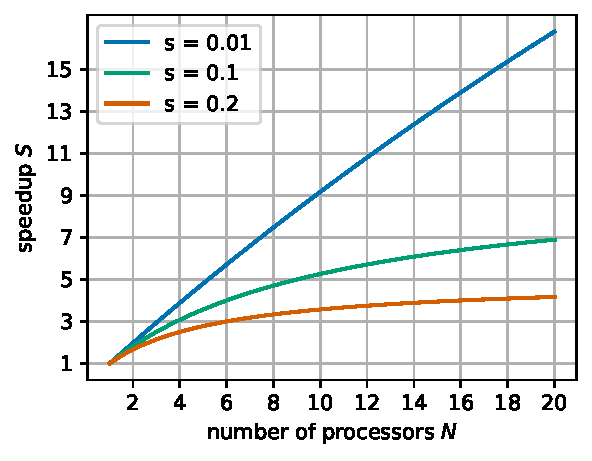
\includegraphics[width=0.9\textwidth]{figs/amdahl.pdf}
				%\caption{Speedup modeled by Amdahl's law for different portions of strictly serial workload}
				\label{fig:ideal_speedup}
			\end{figure}
		\end{column}
	\end{columns}
\end{frame}

\begin{frame}
	\frametitle{Amdahl's Law}
	
	\begin{columns}
		\begin{column}{0.5\textwidth}
			In reality: several factors limiting parallelization

			Simple model given by \emph{Amdahl's law}:
			\begin{itemize}
				\item split serial time into a strictly serial part \(s\) and one which can be parallelized perfectly \(p\)
				\item normalize serial time \(T_1 = s + p = 1\)
				\item execution time on \(N\) processors: \(T_N = s + \frac{p}{N}\)
				\item speedup: \(S = \frac{T_1}{T_N} = \frac{1}{s + \frac{p}{N}} = \frac{1}{s + \frac{1 - s}{N}}\)
				\item relevant features: limited by \(\nicefrac{1}{s}\), for smaller \(s\): closer to linear speedup
			\end{itemize}
		\end{column}

		\begin{column}{0.5\textwidth}
			\begin{figure}
				\centering
				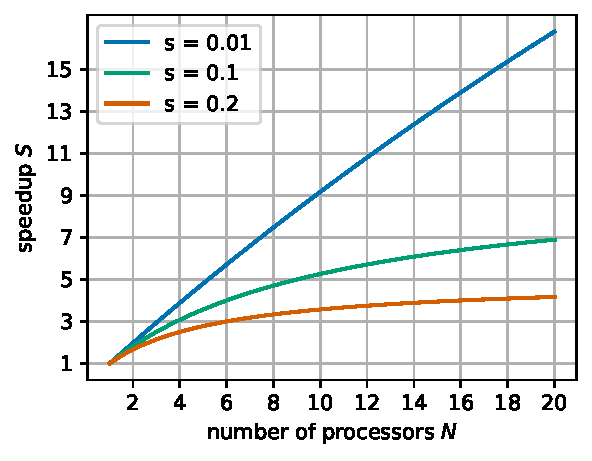
\includegraphics[width=0.9\textwidth]{figs/amdahl.pdf}
				%\caption{Speedup modeled by Amdahl's law for different portions of strictly serial workload}
				\label{fig:amdahl}
			\end{figure}
		\end{column}
	\end{columns}
\end{frame}

\begin{frame}
	\frametitle{}

	\begin{columns}
	\begin{column}{0.5\textwidth}
	\begin{tikzpicture}[
		scale=0.65,transform shape, squarednode/.style={rectangle, draw=purple!60, fill=purple!5, thick, minimum size=5mm, text centered, text width=8cm,},
		node distance=0.5cm]
		\tikzset{every node/.style={inner sep=8pt}}
		%Nodes
		\node[squarednode]      (init)          {Initial \(n(\vb*{r})\)};
		\node[squarednode]      (step_1)    [below= of init]  {Calculate \(v_{\mathrm{H}} [n(\vb*{r})]\) and \(v_{\mathrm{XC}} [n(\vb*{r})]\)};
		\node[squarednode]      (step_2)    [below= of step_1]      {Fourier transform potentials};
		\node[squarednode]      (step_3)    [below= of step_2]      {Solve Kohn-Sham equations in reciprocal space};
		\node[squarednode]      (step_4)    [below= of step_3]      {Fourier transform wave functions};
		\node[squarednode]      (step_5)    [below= of step_4]      {Calculate \(n(\vb*{r})\) and \(E [n(\vb*{r})]\)};
		\node[squarednode]      (done)      [below= of step_5]      {Done if change in \(E\) is small enough};
		
		%Lines
		\draw[->] (init.south) -- (step_1.north);
		\draw[->] (step_1.south) -- (step_2.north);
		\draw[->] (step_2.south) -- (step_3.north);
		\draw[->] (step_3.south) -- (step_4.north);
		\draw[->] (step_4.south) -- (step_5.north);
		\draw[->] (step_5.east) to [out=30,in=-30] (step_1.east);
		\draw[->] (step_5.south) -- (done.north);
	\end{tikzpicture}
	\end{column}

	\begin{column}{0.5\textwidth}
		
	\end{column}

	\end{columns}
\end{frame}

% Folien für Rückfragen

\begin{frame}
	\frametitle{Factors limiting parallel execution}

	

\end{frame}

\end{document}
